%interno poro�ilo
%\documentclass[internal, slovene]{FRIreport}

%zaklju�no poro�ilo
%\documentclass[slovene]{FRIreport}

%seminarska naloga
\documentclass[seminar, slovene]{FRIreport}

% AMS fonts required
\usepackage{iopams}  

% package to include graphics in ps, eps or png format
\usepackage{graphicx}
\usepackage{epstopdf}
% the graphics path
\graphicspath{{img/}}

% define equation referencing
\newcommand{\eqref}[1]{(\ref{#1})}

% define figure referencing
\newcommand{\figref}[1]{\ref{#1}}

% define real numbers symbol
\newcommand{\Rset}{\ensuremath{\mathbb{R}}} 
\newcommand{\R}{\Rset} 
% define natural numbers symbol
\newcommand{\Nset}{\ensuremath{\mathbb{N}}} 
\newcommand{\N}{\Nset} 
% define euclidean vector space symbol
\newcommand{\Eset}{\ensuremath{\mathbb{E}}} 
\newcommand{\E}{\Eset} 

\newcommand{\imp}[1]{{\color{P654M}#1\normalcolor}}

%%%
\newcommand{\angl}[1]{(\textit{angl.} #1)}


\usepackage{tikz}
\usetikzlibrary{shapes.gates.logic.US}
\usetikzlibrary{circuits.logic.US}
\usepackage{circuitikz}

%main
\begin{document}

\title{QCA sekven\v cna ALE}

\author{Miha Zidar, Anže Pečar, Matic Potočnik, Željko Plesac, Jan Varljen}

%\address{Skupina 1}

\begin{abstract}
V seminarju bomo opisali zasnovo sekvenčne ALE s kvantnimi celičnimi avtomati, z uporabo programa QCAdesigner.

\Keywords{kvantni celični avtomati, aritmetično-logična enota, modeliranje in simulacija}
\end{abstract}

%
%%
\section{Uvod}
Predvideva se, da bo že čez nekaj desetletij minituarizacija in zmogljivost čipov, grajenih na siliciju, dosegla končno stopnjo in bo potrebno za večjo procesno moč preiti na drug osnovni material in najverjetneje tudi zelo drugačen pristop k modeliranju vezij. Ena izmed obetajočih alternativ so kvantni celični avtomati \angl{QCA}, ki obljubljajo mnoge prednosti pred klasičinimi vezji:
\begin{itemize}
\item Večnivojska vezja
\item Možnost križanja vodil
\item Enostavna realizacija nekaterih časovnih vezij
\item Potencialno nižja poraba in višji takt delovanja
\item ...
\end{itemize}
V tem seminarju bomo opisali zasnovo sekvenčne ALE, z uporabo odprtokodnega programa QCADesigner\cite{walus:2004}. Sekvenčnost enote tu pomeni, da enota načeloma ne izvaja operacij nad vsebino končno dolgih registrov, ampak sprejema tok(sekvenco) bitov, nad njimi izvaja operacije in kot tok bitov podaja tudi svoj izhod. Kot bomo videli v nadaljevanju, to za določene operacije ni povsem možno in jih interno še vedno realiziramo z registri. Za večino osnovnih operacij pa je sekvenčna implementacija možna in se lepo prilega realizaciji s QCA-ji.

%
%%
\section{Metode}
V tem odseku bomo predstavili nekatere odločitve in metode snovanja, ki smo jih uporabili pri zasnovi naše ALE.

\subsection{Osnovni opis ALE}
Implementiran je logično poln sistem operacij. Za izbiro operacije so uporabljeni trije biti. Naša ALE bo podpirala naslednje operacije:

\begin{center}
\begin{tabular}{ | c | c | c | }\hline
Operacija & Oznaka & Operacijska koda \\ \hline
NOP & $\varnothing$   & 000 \\
NOT & $\lnot$ & 001 \\
AND & $\wedge$ & 010 \\
OR & $\vee$ & 011 \\
SUM & $+$ & 100 \\
SUB & $-$ & 101 \\
MUL & $\times$ & 110 \\
DIV & $\div$ & 111 \\ \hline
\end{tabular}
\end{center}

%
%%
\section{Rezultati}
\subsection{Izbira operacije}
Multiplekser.

\subsection{Vsaka}
\subsection{Operacija}
\subsection{Posebej}


\subsection{Also,vezja}
%shapes.gates.logic.US
%no way, da bi to uporabil...
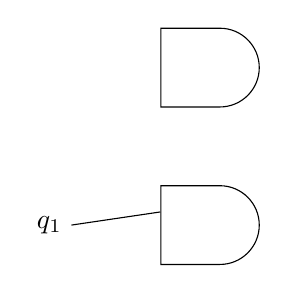
\begin{tikzpicture}[minimum height=1cm]
\node(q1) [] at (0,0) {$q_1$};
\node(and1) [draw, and gate US] at (2,0) {};
\node(and2) [draw, and gate US] at (2,2) {};

\draw (q1.east) -- (and1.input 1);
\end{tikzpicture}
\ \\ \ \\
%circuits.logic.US
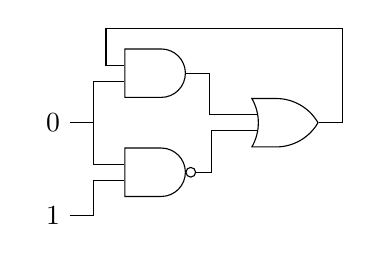
\begin{tikzpicture}[circuit logic US]
\matrix[column sep=7mm]{
		& \node [and gate] (a1) {}; & \\
	\node (i1) {0}; & & \node [or gate] (o) {};\\
		& \node [nand gate] (a2) {}; & \\
	\node (i2) {1}; & & \\
};
\draw 
(i1.east) -- ++(right:3mm) |- (a1.input 2)
(i1.east) -- ++(right:3mm) |- (a2.input 1)
(i2.east) -- ++(right:3mm) |- (a2.input 2)
(a1.output) -- ++(right:3mm) |- (o.input 1)
(a2.output) -- ++(right:2mm) |- (o.input 2)
(o.output) -- ++(right:3mm)
%povezave nazaj so problematične
(o.output) -- ++(right:3mm) -- ++(up:12mm) -- ++(left:30mm) |- (a1.input 1)++(right:3mm)
;
\end{tikzpicture}
\ \\ \ \\
%circuitikz
%(pomojem skor isti način dela kot gor)
\begin{circuitikz}\draw
	(0,2) node[and port] (and1) {}
	(0,0) node[and port] (and2) {}
	(2,1) node[xnor port] (xnor) {}
	
	(and1.in 1) node[anchor=east] {q1}
	(and1.in 2) node[anchor=east] {q2}

	(and1.out) -| (xnor.in 1)
	(and2.out) -| (xnor.in 2)
	%nope
	%(xnor.out) |- (and1.in 2) 
	(and1.in 1)++(0,1) node (and1above) {}
	(xnor.out)++(0,2) node (xorabove) {}
	(xnor.out) |- (xorabove.south) |- (and1above.south) |- (and1.in 1)
;\end{circuitikz}

%
%%
\section{Zaključek}
Zaključi z nekaj izhodišči za nadaljnje delo.

%
%%
\References
%
\bibliographystyle{elsart-num-sl}
%
\bibliography{sample}

\end{document}
